\section{AI辅助幻灯片制作}

在当今数字化时代,随着信息技术的飞速发展,制作一份结构清晰、内容丰富且富有吸引力的PPT已成为教学与学习领域中不可或缺的一项重要技能。无论是课堂教学还是学术研讨,一份高质量的PPT往往能够极大地提升信息传递的效率与效果,帮助学习者更好地理解和掌握知识要点。对于文科生而言,历史学科作为一门研究人类社会发展历程的学科,其知识的深度与广度无疑是至关重要的。历史涵盖了从远古时期到现代社会的诸多方面,包括政治、经济、文化、社会等诸多领域,内容繁杂且相互关联。然而,如何将这些纷繁复杂的历史信息转化为直观、生动的视觉呈现形式,使其更易于被学生接受和理解,常常成为教师和学习者面临的一大挑战。
幸运的是,随着人工智能技术的不断发展,GPT(Generative Pre-trained Transformer)作为一种先进的自然语言处理工具,为这一问题的解决提供了有力的支持。

本节将使用GPT制作高效且美观的通史幻灯片。GPT以其强大的语言生成能力和对海量知识的整合能力,能够帮助我们高效地生成高质量的历史内容。它可以根据用户的需求,快速生成准确、清晰且具有逻辑性的文字内容,无论是对历史事件的详细阐述、对历史人物的深入剖析,还是对历史发展脉络的梳理,都能轻松应对。通过与PPT制作软件的有机结合,GPT能够助力教师和学习者创造出既高效又美观的历史学习材料。借助这一工具,我们可以将枯燥的文字转化为生动的图表、清晰的时间轴、精美的图片以及富有逻辑性的文字布局,从而让历史知识在视觉上更加直观、更具吸引力,极大地提升教学与学习的效果。使用GPT生成幻灯片的过程可描述如下。

首先,制作PPT的第一步是确定主题与大纲。在开始任何创作之前,明确主题是至关重要的。例如,若主题为“中国历史上的重大事件”,则需要围绕这一核心展开内容设计。接下来,设计一个清晰的结构框架,以确保PPT内容的逻辑性和连贯性。可以按照历史朝代划分章节,每个朝代下进一步细化为重要事件、关键人物及其影响等板块。这种结构不仅有助于梳理复杂的历史知识体系,还能使学习者更清晰地把握历史发展的脉络。
在完成主题与大纲的设计后,便可以利用GPT生成内容。打开GPT界面(如ChatGPT),输入具体的请求指令。例如,可以要求生成一份关于“中国历史上的重大事件”的详细大纲,并指定输出格式为Markdown。在提出请求时,务必确保要求具体明确,例如可以指定每部分的字数、是否需要图片说明或关键词等。这样能够使生成的内容更加贴合实际需求,减少后续修改的工作量。

生成内容后,接下来的步骤是整理与优化。将GPT生成的Markdown文本复制到文档中,并仔细检查内容是否符合既定的结构要求。如有必要,对内容进行修改和补充,例如添加特定的历史细节或调整表达方式以适应目标受众的理解水平。这一过程需要结合专业知识和教学目标,确保内容的准确性和适宜性。

完成内容整理后,即可将优化后的Markdown文件导入到PPT制作工具中。目前,许多软件如Mindshow或WPS演示都支持Markdown转换功能。将文件上传后,软件会自动生成PPT,通常包括标题页、各章节内容页和总结页等基本结构。此时,PPT的初步框架已经形成,但为了使其更具吸引力和教学价值,还需要进行进一步的调整与美化。

在调整与美化阶段,可以根据教学需求选择合适的模板,以增强PPT的视觉效果。此外,还可以通过添加图片、图表或时间轴等方式,使内容更加生动形象。例如,在讲述鸦片战争时,插入相关的地图或历史照片,能够帮助学习者更直观地理解事件的背景和影响。这一环节不仅提升了PPT的视觉效果,更有助于增强学习者的兴趣和理解能力。

完成美化后,进入审阅与修改阶段。仔细检查每一页的内容,确保信息准确传达,语言简洁易懂。同时,对引用的历史事件和人物进行必要的核实,确保其准确无误。这一过程需要严谨的学术态度,以保证PPT的学术性和权威性。

最后,将制作完成的PPT用于课堂展示或学习分享,并积极收集同学或老师的反馈意见。根据反馈进一步调整内容或设计,以提升PPT的质量和效果。这一环节不仅有助于完善PPT,还能促进教学方法的改进和提升。
通过以上步骤,结合GPT的强大功能与PPT制作工具的灵活性,我们能够高效地制作出一份结构清晰、内容丰富且具有学术深度的PPT。这不仅为教学活动提供了有力支持,也为学习者创造了更优质的学术体验。

在探讨如何将GPT应用于PPT制作的过程中,我们有必要从实践的角度出发,深入剖析其具体操作流程。这一过程不仅涉及技术层面的应用,更需要结合学术研究的严谨性与教学实践的灵活性,以确保最终生成的PPT既具备学术深度,又符合教学的实际需求。下面从实践的角度具体展示GPT制作``中国古代历史''幻灯片的过程。

\textbf{首先,生成大纲}。向GPT提问:

\prompt{请为我生成一份关于`中国古代历史'的结构化大纲,包括从上古到清朝的重要朝代、关键事件及其影响。}

\begin{gptbox}
% \footnotesize{}
\small{
\begin{lstlisting}[language=Markdown]
      # 中国古代历史
      
      ## 上古时期
      - **三皇五帝**
        - 炎帝神农氏
        - 黄帝轩辕
      - **夏朝**
        - 夏禹建立夏朝
        - 桀的暴政与商汤革命
      
      ## 商周时期
      - **商朝**
        - 盘庚迁殷
        - 武丁中兴
      - **西周**
        - 周公制礼作乐
        - 平王东迁
\end{lstlisting}
}
\end{gptbox}


\textbf{接着,优化内容(可选)}。复制生成的Markdown文本,并根据需要进行调整。例如,补充具体的年份或增加相关的历史评价。


\textbf{然后,生成PPT}
将Markdown上传至WPS演示中的AI模块中,选择一个适合的模板。软件会自动生成包含标题、章节和内容页的PPT, 如\reffig{fig:ppt-wps}至\reffig{fig:ppt-wps-done}所示。

\fig[h]{
      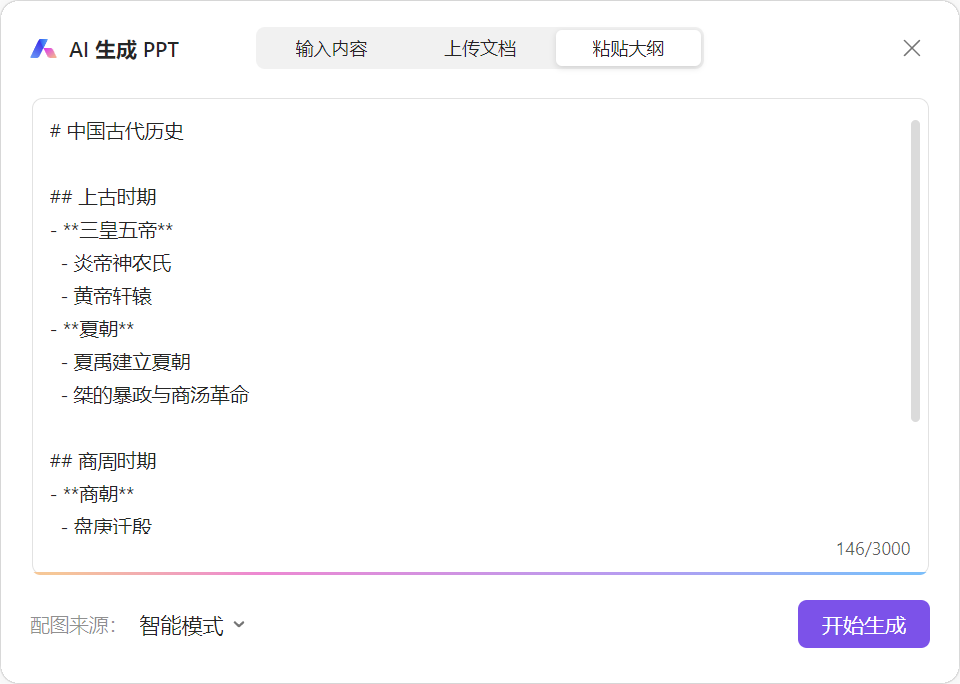
\includegraphics[width=0.7\textwidth]{assets/figures/image-20250210192847219.png} %插入图片,[]中设置图片大小,{}中是图片文件名
      \caption{粘贴大纲到WPS} %最终文档中希望显示的图片标题
      \label{fig:ppt-wps} 
}

\fig[h]{
      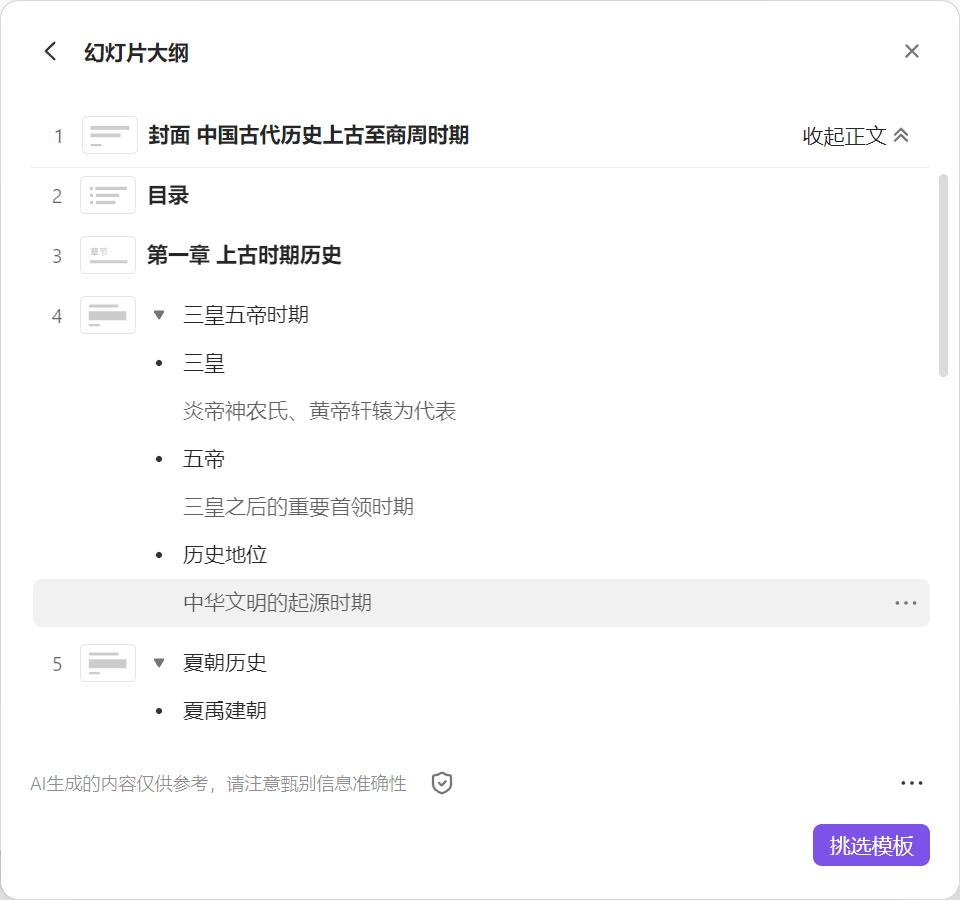
\includegraphics[width=0.7\textwidth]{assets/figures/image-20250210192936323.png} %插入图片,[]中设置图片大小,{}中是图片文件名
      \caption{WPS生成大纲} %最终文档中希望显示的图片标题
      \label{fig:ppt-wps-toc} % 
}

\fig[h]{
      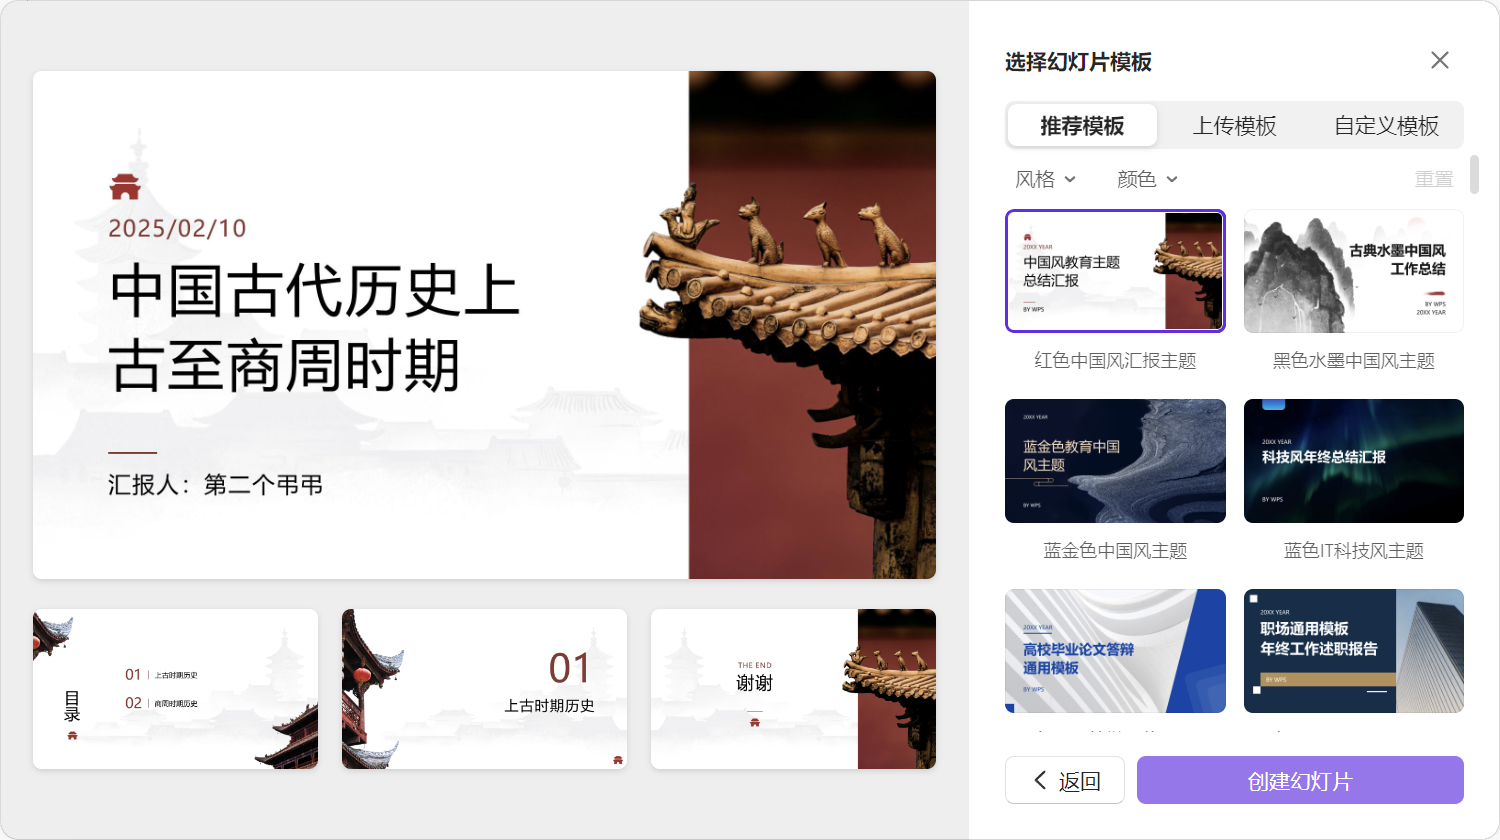
\includegraphics[width=0.7\textwidth]{assets/figures/image-20250210192952252.png} %插入图片,[]中设置图片大小,{}中是图片文件名
      \caption{挑选合适的模板} %最终文档中希望显示的图片标题
      \label{fig:ppt-wps-select} % 
}

\fig[h]{
      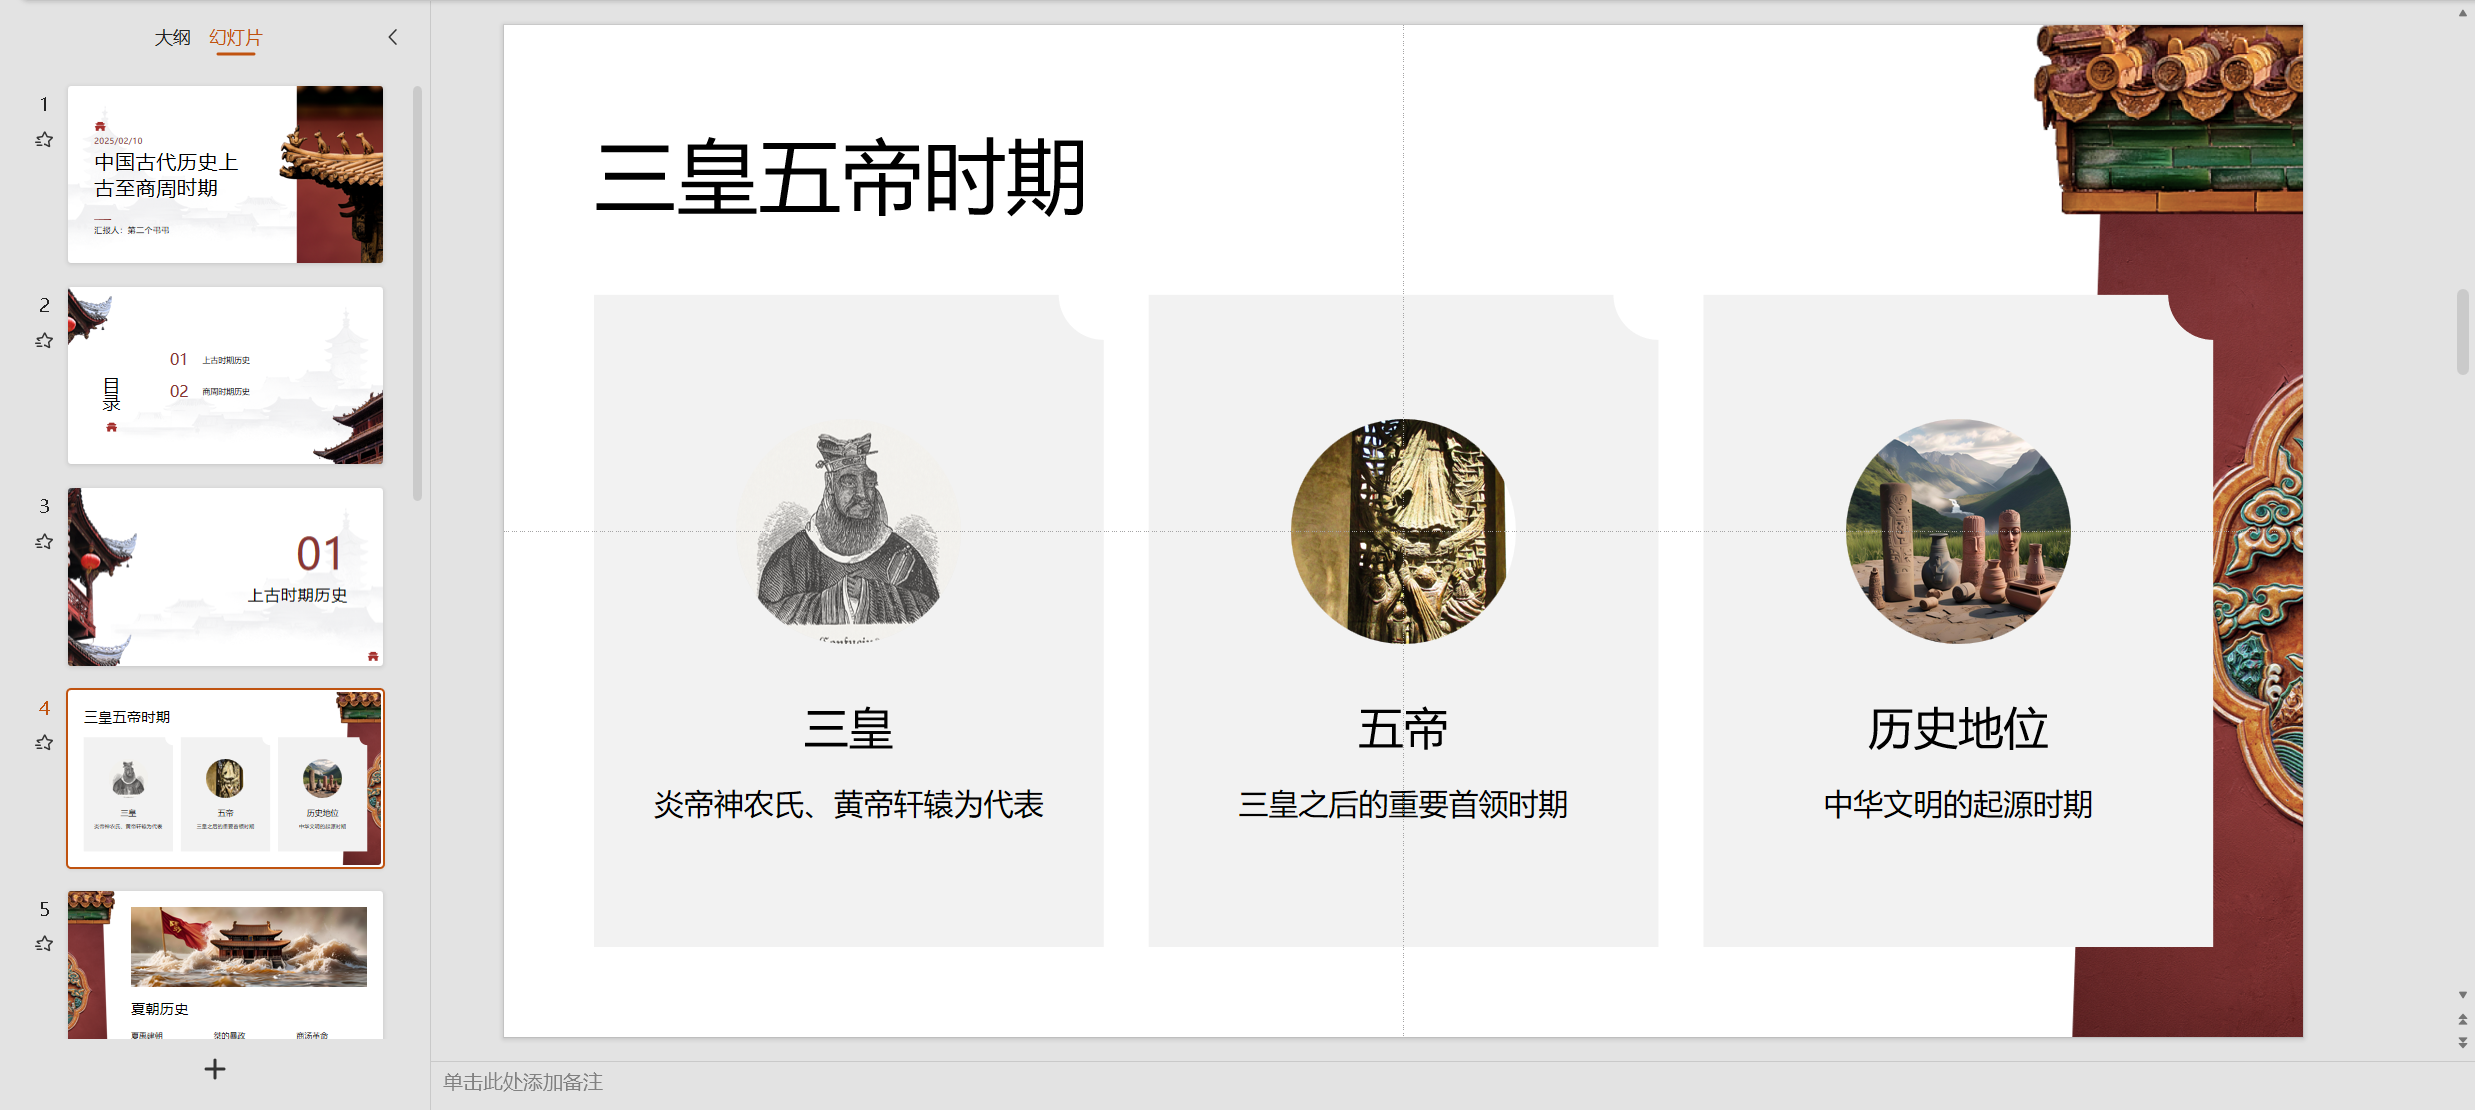
\includegraphics[width=0.7\textwidth]{assets/figures/image-20250210193018631.png} %插入图片,[]中设置图片大小,{}中是图片文件名
      \caption{效果图} %最终文档中希望显示的图片标题
      \label{fig:ppt-wps-done} %用于文内引用的标签 
}

\textbf{最后,美化与调整}。在制作历史主题的PPT时,视觉元素的运用对于增强信息的传达效果至关重要。例如,可以通过添加历史地图或重要人物画像,为观众提供直观的历史背景和人物形象,从而加深对历史情境的理解。此外,使用时间轴来展示各个朝代的更替,能够清晰地呈现历史发展的脉络,帮助观众更好地把握历史事件的时间顺序和相互关系。同时,在关键事件的页面中加入简短的动画效果,不仅可以吸引观众的注意力,还能通过动态呈现增强其对复杂历史过程的理解和记忆。这些设计手段不仅丰富了PPT的视觉效果,更在学术表达上提升了内容的可读性和教育价值。

综上,通过GPT生成结构化的内容,并结合专业的PPT制作工具,我们可以高效地创建出内容丰富、设计美观的历史PPT。这种方法不仅节省时间,还能确保信息的准确性和呈现的专业性,特别适合文科生在学习和教学中使用。随着技术的发展,未来的工具将更加智能,帮助我们更轻松地完成复杂的任务。

值得一提的是,在运用GPT生成历史相关内容时,常会面临一些关键性问题,而这些问题的妥善解决对于保证学术性和教学效果至关重要。首先,关于内容的准确性问题,尽管GPT具备强大的信息生成能力,但在处理历史知识时,仍需谨慎对待。历史学科的严谨性要求我们在使用生成的内容后,必须进行仔细的校对,并参考权威的历史资料加以验证。通过这一过程,可以有效避免因技术生成的偏差而带来的错误信息,确保内容的科学性和可靠性。
其次,面对复杂的主题,如何有效处理也是一个重要问题。历史学科中不乏内容丰富且层次复杂的主题,如某一历史时期的变革或某一重大事件的多维度影响。在这种情况下,可以采用分步查询的方法,逐步向GPT提出细化的问题,从而逐步完善每个部分的内容。通过这种方式,能够确保在生成内容时,结构清晰、逻辑连贯,避免因内容过于庞杂而导致的混乱。这种分步细化的策略不仅有助于提高内容的质量,也使得历史知识的呈现更加条理化,便于学习者理解和接受。
